% CSC officers
\documentclass[11pt]{article}
\usepackage[margin=0.7in]{geometry}
\usepackage{listings}   %
\usepackage{needspace}  %
\usepackage{color}      %
\usepackage{ifthen}     % 
\usepackage{graphicx}   %
\usepackage{csc}        %
\usepackage{tikz}       %
\usetikzlibrary{shapes, arrows, automata} %
\usepackage{tabularx}   % for helping matchtabular (matching questions)
\usepackage{textcomp}	% So our quotes in code don't look like shit
\usepackage{longtable}
\usepackage{multicol}
\usepackage{tabu}
\setlength{\columnsep}{12em}

\lstset{ %
basicstyle=\footnotesize\ttfamily,       % the size of the fonts that are used for the code
numbers=left,                   % where to put the line-numbers
stepnumber=1,                   % the step between two line-numbers. If it's 1 each line will be numbered
numbersep=5pt,                  % how far the line-numbers are from the code
showspaces=false,               % show spaces adding particular underscores
showstringspaces=false,         % underline spaces within strings
tabsize=4,		                % sets default tabsize to 4 spaces
language=Java,
upquote=true,
columns=fixed
}

\ifthenelse{\isundefined{\isAnswerKey}}
{
    \newenvironment{answer}{\large\lstset{basicstyle=\tiny\ttfamily}\color{white} }{}
}
{
    \newenvironment{answer}{\large\lstset{basicstyle=\footnotesize\ttfamily}\color{red} }{}
}

\ifthenelse{\isundefined{\isAnswerKey}}
{
	\newcommand{\answerrow}[1]{\hline \rowfont{\color{white}} #1}
}
{
	\newcommand{\answerrow}[1]{\hline \rowfont{\color{red}} #1}
}

% ----- Start matchtabular definition -----
\newcounter{matchleft}
\newcounter{matchright}
\newenvironment{matchtabular}{%
  \setcounter{matchleft}{0}%
  \setcounter{matchright}{0}%
  \tabularx{\textwidth}{%
    >{\leavevmode\hbox to 1.5em{\stepcounter{matchleft}\arabic{matchleft}.}}X%
    >{\leavevmode\hbox to 1.5em{\stepcounter{matchright}\alph{matchright})}}X% 
    }%
}{\endtabularx}
% ----- End matchtabular definition -----

\title{CSCI-142 Exam 2 Review}
\author{Computer Science Community}
\date{\today}

\makeatletter
\let\thetitle\@title
\let\theauthor\@author
\let\thedate\@date
\makeatother

\begin{document}
\header
\begin{enumerate}

\item Suppose we are talking about the depth-first search (DFS) algorithm. Nodes are added to the data structures in alphabetical order.
\begin{enumerate}
\item What underlying data structure does this algorithm use?

\begin{answer}
A stack.
\end{answer}

\item
Given the following graph, state the DFS traversal order and show the data structure at each step.
Node \texttt{A} is the start node, and \texttt{F} is the destination node.

\begin{minipage}{0.35\textwidth}
\vspace{-136pt}
\begin{answer}
$\leftarrow$ bottom of stack \\
\textbar A \\
\textbar B C \\
\textbar B D E \\
\textbar B D \\
\textbar B F \\
\textbar B \\

The traversal order is ACEDF.
\end{answer}
\end{minipage}
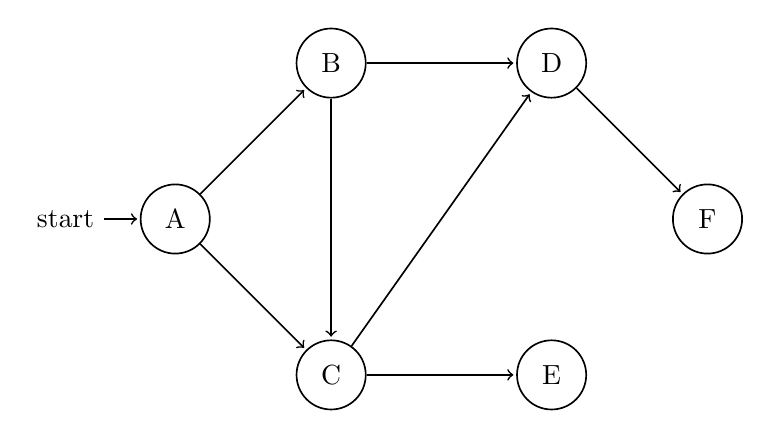
\begin{tikzpicture}[shorten >=1pt,auto,node distance=2.8cm,semithick]
	\node[initial,state] (A) {A};
	\node[state]        (B) [above right of=A] {B};
	\node[state]        (C) [below right of=A] {C};
	\node[state]        (D) [right of=B] {D};
	\node[state]        (E) [right of=C] {E};
	\node[state]        (F) [below right of=D] {F};

	\path[->]   (A) edge node {} (C)
		(A) edge node {} (B)
		(B) edge node {} (C)
		(B) edge node {} (D)
		(C) edge node {} (D)
		(C) edge node {} (E)
		(D) edge node {} (F);
\end{tikzpicture}

\item
What path from \texttt{A} to \texttt{F} does the DFS algorithm return?

\begin{answer}
ACDF 
\end{answer}

\end{enumerate}


\item Now consider a BFS algorithm, again populating data structures in alphabetical order.
\begin{enumerate}
\item
What changes would need to be made to a DFS implementation to turn it into a breadth-first search (BFS)?

\begin{answer}
Use a queue data structure (instead of a stack).
\end{answer}

\item
Using the graph as described in Question 1, what is the BFS traversal order?
Show the data structure at each step. \\
\begin{answer}
$\leftarrow$ front of queue \\
A \\
B C \\
C D \\
D E \\
E F \\
F \\

The traversal order is ABCDEF.
\end{answer}

\item
What path from \texttt{A} to \texttt{F} results from the BFS algorithm?

\begin{answer}
ABDF
\end{answer}

\end{enumerate}

\newpage
\item \textbf{Searching a Graph}
	\begin{enumerate}
		\item
			Write a recursive algorithm that (given a graph, start vertex, and goal vertex),
			determines whether or not there is a path to the goal vertex.

            Assume you are provided with a \texttt{Graph} class with a \texttt{getNeighbors( int vertex )} method, which returns a \texttt{Set\textless Integer\textgreater} representing the numbers corresponding to neighboring vertices. Assume \texttt{visited} is a \texttt{Set} keeping track of all visited vertices. \\
			(Note: Your algorithm should return a Boolean value, not an actual path!)
\begin{verbatim}
boolean hasPathToRec(Graph g, int start, int goal, Set<Integer> visited) {
\end{verbatim}
			
\begin{answer}
\begin{lstlisting}
	if( start == goal ){
		return true;
	} else {
		for( int n : g.getNeighbors(start) ){
			if( ! visited.contains(n) ){
				visited.add(n);
				if ( hasPathToRec(g, n, goal, visited) )
					return true;
			}
		}
		return false;
	}
}
\end{lstlisting}
\end{answer}
		            
		\item
			Rewrite your algorithm to be iterative instead. \\
			(Hint: What data structure do you need to use if you no longer have recursion?)
\begin{verbatim}
boolean hasPathToIter(Graph g, int start, int goal, Set<Integer> visited) {
\end{verbatim}	
			
\begin{answer}
\begin{lstlisting}
	Stack<Integer> theStack = new Stack<Integer>();
	theStack.push(start);
	visited.add(start);
	while( ! theStack.empty() ){
		int curr = theStack.pop();
		if( curr == goal ){
			return true;
		}
		for( int n : g.getNeighbors(curr) ){
			if( ! visited.contains(n) ) {
				visited.add(n);
				theStack.push(n);
			}
		}
	}
	return false;
}
\end{lstlisting}
\end{answer}
	\end{enumerate}


\item When is a vertex's sum weight finalized in Dijkstra's algorithm?

    \begin{answer}
    A vertex's sum weight is final after it has updated the tentative distances
    of all of its neighbors. As part of being finalized, it's moved from the
    unvisited set to the visited set.
    \end{answer}

\item What role does the priority queue play in finding the shortest path?
      When do we use it?

    \begin{answer}
    The priority queue is used to select the next vertex to visit. We want to
    visit the node which currently has the lowest tentative distance from the
    start, so we use a priority queue that always returns the lowest element.
    \end{answer}

\newpage
\item Why does Dijkstra's algorithm not work correctly on graphs with negative
      edge weights?

\begin{answer}
Dijkstra's algorithm doesn't work correctly on graphs with negative edge
weights due to one of its {\em greedy} behaviors.

When selecting the next node to visit, Dijkstra's algorithm chooses the
node with the current lowest total value, then {\em finalizes} that value
forever. If there were another route to that node, which had not yet been
explored (and contained a net negative weight) Dijkstra's algorithm would
return a suboptimal path.
\end{answer}


\vspace{24pt}

\item Consider the following graph. \\
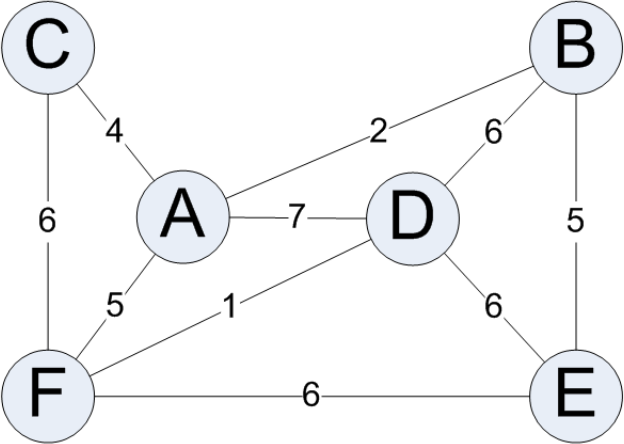
\includegraphics[height=150px]{other/graph.png}
\begin{enumerate}
	\item
	Perform Dijkstra's algorithm to find the shortest path between C and E. \\
	\def\arraystretch{1.65}
	\begin{tabu}{| c | c | c | c | c | c | c |}
		\hline
		Finalized & A & B & C & D & E & F\\
		\hline
		-- & ($\infty$, None) & ($\infty$, None) & \textbf{(0, None)} & ($\infty$, None) & ($\infty$, None) & ($\infty$, None) \\
		\answerrow{C & \textbf{(4, C)} & ($\infty$, None) & (0, None) & ($\infty$, None) & ($\infty$, None) & \textbf{(6, C)}} \\
		\answerrow{A & (4, C) & \textbf{(6, A)} & (0, None) & \textbf{(11, A)} & ($\infty$, None) & (6, C)} \\
		\answerrow{F & (4, C) & (6, A) & (0, None) & \textbf{(7, F)} & \textbf{(12, F)} & (6, C)} \\
		\answerrow{B & (4, C) & (6, A) & (0, None) & (7, F) & \textbf{(11, B)} & (6, C)} \\
		\answerrow{D & (4, C) & (6, A) & (0, None) & (7, F) & (11, B) & (6, C)} \\
		\answerrow{E & (4, C) & (6, A) & (0, None) & (7, F) & (11, B) & (6, C)} \\
		\hline
	\end{tabu} \\

	\begin{answer}
		The shortest path is CABE with a total cost of 11.
		To reconstruct this solution, we start with the destination node, then move on to its recorded optimal predecessor.
		We repeat the process until we reach the starting node.
		(Note that this isn't the only possible table.)
	\end{answer}

	\item
	In general, when using Dijkstra's algorithm to find the shortest path between nodes,
	do you need to use every row of the table? Why or why not?

	\begin{answer}
		No. The algorithm is finished as soon as the destination node has been finalized;
		Dijkstra's is a greedy algorithm so it will never change decisions once they are made.
	\end{answer}
\end{enumerate}


\newpage
\item Explain the Model-View-Controller design pattern. \\
\begin{answer}
MVC is a way of dividing responsibility within a project's code to prevent it from growing intertwined to the point of unmaintainability.
The model is the portion of the code that manages storing, representing, and manipulating the data.
The controller is the module that accepts user input and prepares it for use by the model.
The view describes the appearance of the user interface.
\end{answer}

\item Describe each of the following layout managers:
\begin{enumerate}

\item \texttt{FlowPane}
\begin{answer}
The \texttt{FlowPane} class puts components in a row, sized at their preferred size. If the horizontal space in the container is too small to put all the components in one row, the \texttt{FlowPane} class uses multiple rows. If the container is wider than necessary for a row of components, elements in the row will be flushed left by default. \end{answer}

\item \texttt{BorderPane}
\begin{answer}
\texttt{BorderPanes} allow you to specify the positional location to place new elements into the pane, including top, center, bottom, left, and right. You can specify where to put elements by \texttt{paneName.set[Position](Node value)}. Elements that are placed in the scene will retain their size if there is enough space.\end{answer}

\item \texttt{GridPane}
\begin{answer}
A \texttt{GridPane} places components in a grid of cells. The largest component in any given row or column dictates the size of that row or column, meaning if all your components are the same size, all the grid cells in the pane will be the same size.\end{answer} 

\item \texttt{HBox and VBox}
\begin{answer}
An \texttt{HBox} places its components horizonally left-to-right.
A \texttt{VBox} is like an \texttt{HBox} except that it adds components vertically top-to-bottom.
\end{answer}

\end{enumerate}

\vspace{24pt}


\item Write a function or routine which creates a \texttt{Button} with the text "Click me!" that prints out a message of your choosing when it is clicked, using \texttt{System.out.println()}. When you've reached a solution, think about how you might be able to reorganize the code which tells the button what do when it is pressed in a different way.

\begin{answer}

\lstinputlisting{code/event_listener_code.java}

\end{answer}



\newpage
\item Create a class that constructs and displays the following GUI. If you can't remember exactly how to implement a certain part of the GUI in code, explain what the component is and how it would fit in with the rest of the calculator. (\textit{Hint: draw out the GUI's \textbf{component hierarchy}.})\\
%image is right-aligned to give students more writing space
\begin{minipage}{0.5\textwidth}
\vspace{-54pt}
The buttons within the GUI do not need to be functional.  You may or may not need the following: \texttt{Scene}, \texttt{BorderPane}, \texttt{FlowPane}, \texttt{HBox}, \texttt{TextField}, \texttt{Button}. The window should fit to all of the components and have a title.
\end{minipage}
\hspace{50px}
\begin{minipage}{0.3\textwidth}
\vspace{6pt}
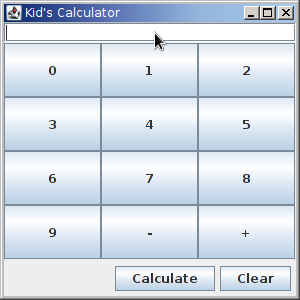
\includegraphics[scale=0.6]{other/calculator.png}
\end{minipage} \hfill

\vspace{-60pt}
\begin{answer}
\begin{lstlisting}[language=java,basicstyle=\scriptsize]
public class KidsCalc extends Application {
    private final static int BUTTON_WIDTH = 80;
    private final static int BUTTON_HEIGHT = 50;
    private final static int MIN_WIDTH = BUTTON_WIDTH*3;

    public void start(Stage primaryStage) throws Exception {
        Scene scene = new Scene(this.makeMainPane());
        primaryStage.setTitle("Kid's Calculator");
        primaryStage.setScene(scene);
        primaryStage.show();
    }

    private Parent makeMainPane() {
        BorderPane bp = new BorderPane();	//BORDER PANE LAYOUT
        bp.setPrefWidth(MIN_WIDTH);
        bp.setTop(makeTopArea()); 		//TOP
        bp.setCenter(makeCenterArea());	//CENTER
        bp.setBottom(makeBottomArea());	//BOTTOM
        return bp;
    }

    private Node makeTopArea(){
        TextField t = new TextField("0");
        t.setEditable(false);
        return t;
    }

    private Node makeCenterArea(){
        FlowPane flow = new FlowPane();
        flow.setMinWidth(MIN_WIDTH);
        
        for(int i = 0; i<10; i++){	// buttons 0 - 9
            Button b = new Button(String.valueOf(i));
            b.setPrefSize(BUTTON_WIDTH,BUTTON_HEIGHT);
            flow.getChildren().add(b);
        }
        
        Button minus = new Button("-"); 
        minus.setPrefSize(BUTTON_WIDTH,BUTTON_HEIGHT);
        flow.getChildren().add(minus);
        Button plus = new Button("+");
        plus.setPrefSize(BUTTON_WIDTH, BUTTON_HEIGHT);
        flow.getChildren().add(plus);
        return flow;
    }

    private Node makeBottomArea(){
        HBox bottom = new HBox(8);				//HBox for bottom row
        bottom.setAlignment(Pos.CENTER_RIGHT);
        Button calculate = new Button("Calculate");	//calculate button
        bottom.getChildren().add(calculate);
        Button clear = new Button("Clear");			//clear button
        bottom.getChildren().add(clear);
        return bottom;
    }
}
\end{lstlisting}
\end{answer}


\newpage
\item Briefly explain the differences between the three kinds of exceptions: checked exceptions, runtime exceptions, and errors.
\begin{answer}

\textbf{checked exceptions} -� Exceptions that a method signature must specify it throws. If a method
may throw a checked exception, all calls to that method must be within a \texttt{try}-\texttt{catch} block. Checked exceptions should be used exclusively for foreseeable runtime mistakes, and any reasonably robust
system should be able to recover from one. Classic example is \texttt{IOException}.\\

\textbf{runtime exception} -� Not declared in a method signature and not anticipated to be thrown.
Usually arise due to software bugs and often cause the program to crash. Classic
examples are \texttt{NullPointerException} and \texttt{ArrayIndexOutOfBoundsException}.\\

\textbf{errors} -� Represent a serious issue outside of the control of the programmer (hard drive
failure, not enough memory, device issue). Examples are \texttt{IOError}, \texttt{VirtualMachineError} and
\texttt{ThreadDeath} (see Java's \texttt{Error} class).
\end{answer}


\vspace{48pt}

\item Is there anything wrong with the following exception handler as written? Will this
code work as intended? 
\begin{lstlisting}[language=java]
try {
	this.epicFail();
} catch (Exception e) {
	...
} catch (ArithmeticException a) {
	...
}
\end{lstlisting}
\begin{answer}
\texttt{Exception} is more broad than \texttt{ArithmeticException}, so the second \texttt{catch} statement is unreachable.  \texttt{catch} statements should filter possible \texttt{Exception} types from specific to broad.
\end{answer}

\newpage
\item What is the output when \texttt{LookAtDatMagic}'s main is executed?
\begin{lstlisting}
public class HeySteve{
    public int bananza(int in) throws NewException{
        if ( in == 7 ){
            throw new NewException("HeySteve, cut that out!");
        }
        return in;
    }
}

public class NewException extends Exception{
    public NewException(String message){
        super(message);
    }

}
           
public class WakaWaka{
    public String BeachBash(Object a, Object b) throws NewException{
        if ( a.equals(b) ){
            throw new NewException("It's a Beach-bash! WakaWaka!");
        }
        return "Da-nanananan";
    }
}

public class LookAtDatMagic{
    public void magic() throws NewException{
        int maraca = 5;
        try{
            HeySteve steve = new HeySteve();
            maraca = steve.bananza(7);
        }catch(NewException e){
            System.out.println(e.getMessage());
        }finally{
            WakaWaka waka = new WakaWaka();
            System.out.println(waka.BeachBash(maraca, 5));
        }
    }

    public static void main(String[] args){
        try{
            LookAtDatMagic ladm = new LookAtDatMagic();
            ladm.magic();
        }catch(NewException e){
            System.out.println(e.getMessage());
        }
    }
}


\end{lstlisting}
\begin{answer}
HeySteve, cut that out!


It's a Beach-bash! WakaWaka!
\end{answer}

\newpage
\item Consider a simple backtracking algorithm.

\begin{enumerate}
\item What are the four core components of any backtracking \texttt{solve} function?

\begin{answer}
\begin{enumerate}
\item
Checking if the current state is the solution - \texttt{isGoal()}, 
\item
Getting the next possible state - \texttt{getSuccessors()}, 
\item
Checking if the next state is valid - \texttt{isValid()}, 
\item
Calling solve on the new valid state - \texttt{solve()}
\end{enumerate}
\end{answer}

\item Write a generic \texttt{solve()} function for a given configuration, which returns either the solution configuration or \texttt{null} (if no solution exists): \\
(\textit{Hint: make up a function name for each of the parts above, if necessary})
\vspace{.25in}
\begin{lstlisting}[numbers=none]
public Configuration solve(Configuration config) {
\end{lstlisting}
\begin{answer}
\begin{lstlisting}[numbers=none]
	if(config.isGoal()){
		return config;
	}else{
		for(Configuration child : config.getSuccessors()){
			if(child.isValid()){
				Configuration ans = solve(child);
				if(ans != null)
					return ans;
			}
		}
		// implicit backtracking happens here
	}
	return null;
\end{lstlisting}
\end{answer}
\begin{lstlisting}[numbers=none]
}
\end{lstlisting}
\end{enumerate}


\end{enumerate}
\end{document}

Topics for this exam:
	- Graphs: (I)DFS/BFS
	- Dijkstra's
	- Intro. to GUIs (from OO perspective)
	- Event-Driven Programming
	- Swing (& Swing Threading)
	- Exceptions
	- Backtracking


